%This work is licensed under the Creative Commons License Attribution 4.0 International (CC-BY 4.0)
%https://creativecommons.org/licenses/by/4.0/legalcode
\documentclass[rgb]{standalone}
\usepackage{tkz-euclide}
\usepackage{amsmath}
\definecolor{myorange}{hsb}{0.0833, 1, 0.8}
\definecolor{mygreen}{hsb}{0.3333, 1, 0.8}
\definecolor{myblue}{hsb}{0.5833, 1, 0.8}
\definecolor{mymagenta}{hsb}{0.8333, 1, 0.8}
\begin{document}
	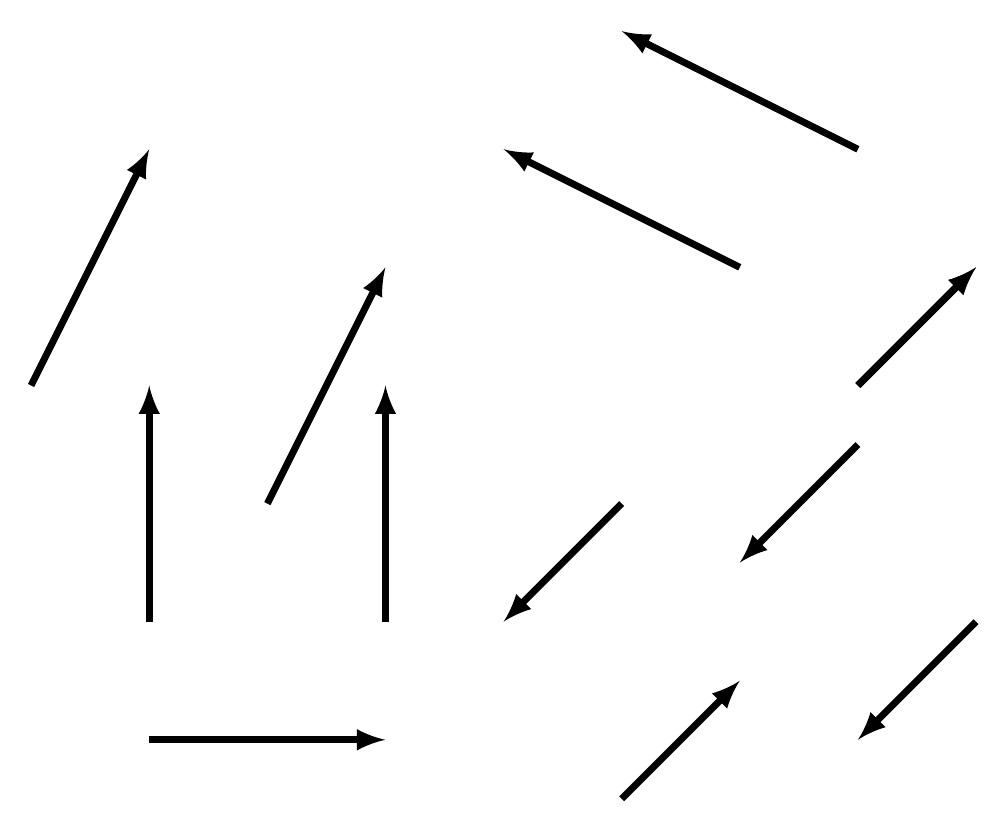
\begin{tikzpicture}[scale=1.5, font=\Large]
		\draw[line width=2.5pt,-latex] (0,0) -- (0,2);
		\draw[line width=2.5pt,-latex] (2,0) -- (2,2);
		\draw[line width=2.5pt,-latex] (-1,2) -- (0,4);
		\draw[line width=2.5pt,-latex] (1,1) -- (2,3);
		\draw[line width=2.5pt,-latex] (0,-1) -- (2,-1);
		\draw[line width=2.5pt,-latex] (5,3) -- (3,4);
		\draw[line width=2.5pt,-latex] (6,4) -- (4,5);
		\draw[line width=2.5pt,-latex] (4,-1.5) -- (5,-0.5);
		\draw[line width=2.5pt,-latex] (6,2) -- (7,3);
		\draw[line width=2.5pt,-latex] (6,2) -- (7,3);
		\draw[line width=2.5pt,-latex] (4,1) -- (3,0);
		\draw[line width=2.5pt,-latex] (7,0) -- (6,-1);
		\draw[line width=2.5pt,-latex] (6,1.5) -- (5,0.5);
	\end{tikzpicture}
\end{document}